% 定义画圈命令,用于标记主元
\newcommand{\circlednum}[1]{%
    \tikz[baseline=(char.base)]{%
        \node[draw, circle, inner sep=1pt] (char) {#1};%
    }%
}

\section{一般线性系统与阶梯形式}
正如我们在前一节中提到的,解线性方程组的方法是将其转化为增广矩阵,使用初等行变换将增广矩阵化简,然后解由简化矩阵表示的等价系统。这个过程如下图所示。

\begin{figure}[h]
    \centering
    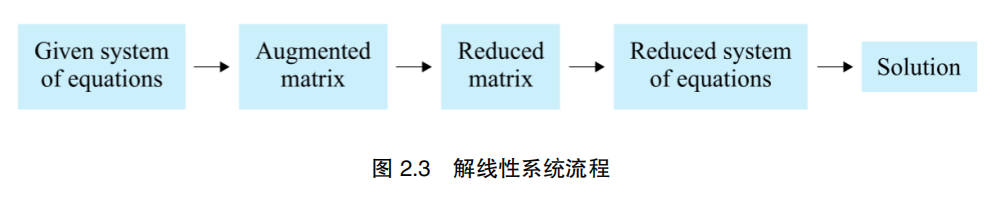
\includegraphics[width=\linewidth]{../images/2.1-1.png} % 请根据实际情况替换图片路径
    \caption{解线性系统流程}
    \label{fig:linear_system_process}
\end{figure}

我们了解了对于 \(n \times n\) 矩阵进行高斯消去的相关内容,这对应于有 \(n\) 个方程和 \(n\) 个未知数的情况。但是如果我们要推广到更一般的线性系统,该如何操作呢?在本节中,我们将介绍更一般的高斯消去法,给出一般线性系统矩阵的行阶梯形式。

我们的第一个目标是将高斯消元技术从方程组扩展到完全通用的矩形系统即线性系统方程的个数与变量的个数不相等的情况。回顾一下,对于具有唯一解的方程组,主元的位置总是位于系数矩阵 \(A\) 的主对角线上- 即从左上角到右下角的对角线上。这样做可以确保高斯消元导致 \(A\) 被减小为一个三角矩阵。以 \(n=4\) 为例,如下图所示:
\[
T=\begin{pmatrix} 
\circledast & * & * & * \\ 
0 & \circledast & * & * \\ 
0 & 0 & \circledast & * \\ 
0 & 0 & 0 & \circledast 
\end{pmatrix}
\]
我们知道主元必须是非零数。对于具有唯一解的方阵系统,我们总是可以在主对角线上的每个关键位置引入一个非零数。然而,在一般矩形系统的情况下,在系数矩阵中并不总是可能使主元位置位于一条直线上。这意味着高斯消去的最终结果不会是三角形的。例如,考虑以下系统:
\[
\begin{cases} 
x_{1}+2 x_{2}+x_{3}+3 x_{4}+3 x_{5}=5 \\ 
2 x_{1}+4 x_{2}+4 x_{4}+4 x_{5}=6 \\ 
x_{1}+2 x_{2}+3 x_{3}+5 x_{4}+5 x_{5}=9 \\ 
2 x_{1}+4 x_{2}+4 x_{4}+7 x_{5}=9 
\end{cases}
\]
该系统的系数矩阵为:
\[
A=\begin{pmatrix} 
1 & 2 & 1 & 3 & 3 \\ 
2 & 4 & 0 & 4 & 4 \\ 
1 & 2 & 3 & 5 & 5 \\ 
2 & 4 & 0 & 4 & 7 
\end{pmatrix}
\]
对系数矩阵 \(A\) 应用高斯消去法得到如下形式:
\[
\begin{pmatrix} 
\circlednum{1} & 2 & 1 & 3 & 3 \\ 
2 & 4 & 0 & 4 & 4 \\ 
1 & 2 & 3 & 5 & 5 \\ 
2 & 4 & 0 & 4 & 7 
\end{pmatrix}
\to
\begin{pmatrix} 
1 & 2 & 1 & 3 & 3 \\ 
0 & \circlednum{0} & -2 & -2 & -2 \\ 
0 & 0 & 2 & 2 & 2 \\ 
0 & 0 & -2 & -2 & 1 
\end{pmatrix}
\]
在之前所讨论的高斯消去的过程中,从第一行开始向下然后向右进行消除,如果向右移动下一个位置进行消除时,此时该位置元素为0,这时则执行与该位置所在行以下的行的交换,以便将非零数带入该位置。但是,在本例中,显然不可能通过将第二行与较低的行互换来将非零数带入 \((2,2)\) 位置。

\subsection{高斯消去法的改进与行阶梯型(Row Echelon Form)}
我们知道在一般矩形系统的情况下,对系数矩阵作高斯消去时在矩阵中并不总是可能使主元位置位于一条对角直线上。这意味着高斯消去的最终结果不会是三角形式。为了处理这种情况,我们对高斯消去做了一定的修改。

\begin{bluebox}{修正后的高斯消元法}
假设 \(U\) 是第 \(i-1\) 步高斯消去后的系统增广矩阵。执行第 \(i\) 步的步骤如下:
\begin{itemize}
    \item 在 \(U\) 中从左到右移动,找到第 \(i\) 个非零位置或该位置下面包含非零元素的那一列,我们把这一列写作 \(U_{* j}\)。
    \item 第 \(i\) 步高斯消去后的主元位置是在 \((i, j)\)。
    \item 如果 \((i, j)\) 的元素为0,则可以将第 \(i\) 行与下面的非零行交换,将一个非零数带入 \((i, j)\) 位置,然后消去这个主元以下的所有元素。
    \item 如果行 \(U_{i *}\) 以及下面 \(U\) 中的所有行都是零,那么消除过程就完成了。
\end{itemize}
\end{bluebox}

% 红色文字
\textcolor{red}{例子2.1.1}
% 红色水平线(宽度为文本宽度,厚度0.4pt)
\color{red}\rule{\textwidth}{0.4pt}\color{black}

对以下矩阵应用修正高斯消去法,圈出支点位置:
\[
A=\begin{pmatrix} 
1 & 2 & 1 & 3 & 3 \\ 
2 & 4 & 0 & 4 & 4 \\ 
1 & 2 & 3 & 5 & 5 \\ 
2 & 4 & 0 & 4 & 7 
\end{pmatrix}
\]
解答:
\[
\begin{pmatrix} 
\circlednum{1} & 2 & 1 & 3 & 3 \\ 
2 & 4 & 0 & 4 & 4 \\ 
1 & 2 & 3 & 5 & 5 \\ 
2 & 4 & 0 & 4 & 7 
\end{pmatrix}
\to
\begin{pmatrix} 
\circlednum{1} & 2 & 1 & 3 & 3 \\ 
0 & 0 & \circlednum{2} & -2 & -2 \\ 
0 & 0 & 2 & 2 & 2 \\ 
0 & 0 & -2 & -2 & 1 
\end{pmatrix}
\]

\[
\to
\begin{pmatrix} 
\circlednum{1} & 2 & 1 & 3 & 3 \\ 
0 & 0 & \circlednum{2} & -2 & -2 \\ 
0 & 0 & 0 & 0 & \circlednum{0} \\ 
0 & 0 & 0 & 0 & 3 
\end{pmatrix}
\to
\begin{pmatrix} 
\circlednum{1} & 2 & 1 & 3 & 3 \\ 
0 & 0 & \circlednum{2} & -2 & -2 \\ 
0 & 0 & 0 & 0 & \circlednum{3} \\ 
0 & 0 & 0 & 0 & 0 
\end{pmatrix}
\]
上面的例子中应用高斯消去的最终结果不是一个纯粹的三角形形式,而是一个锯齿状或"阶梯"类型的三角形形式。此后,具有这种阶梯结构的矩阵将被称为行阶梯形式。

\begin{bluebox}{修正后的高斯消元法}
一个 \(m \times n\) 矩阵 \(E\),其行 \(E_{i *}\),列 \(E_{* j}\) 被称为行阶梯形,满足下面两个条件:
\begin{itemize}
    \item 如果 \(E_{i *}\) 全部由0组成,那么 \(E_{i}\) 下面的所有行也全部为0,即所有的零行都在 \(E\) 底部。
    \item 如果 \(E_{i}\) 中的第一个非零项在第 \(j\) 个位置,那么在这之前的所有列在 \(E_{* 1}, E_{* 2}, \cdots, E_{* j}\) 中第 \(i\) 行位置以下的项全为0。
\end{itemize}
\end{bluebox}

这两个条件说明,行阶梯形中的非零元素必须位于或高于一条阶梯线,这条线从左上角开始,并向右向下倾斜。主元是每一行的第一个非零项。行阶梯形矩阵的典型结构如下图所示:
\[
\begin{pmatrix} 
\circledast & * & * & * & * & * & * & * \\ 
0 & 0 & \circledast & * & * & * & * & * \\ 
0 & 0 & 0 & \circledast & * & * & * & * \\ 
0 & 0 & 0 & 0 & 0 & 0 & \circledast & * \\ 
0 & 0 & 0 & 0 & 0 & 0 & 0 & 0 \\ 
0 & 0 & 0 & 0 & 0 & 0 & 0 & 0 
\end{pmatrix}
\]
由于选择行变换将矩阵 \(A\) 简化为行阶梯形 \(E\) 的灵活性, \(E\) 中的元素不是唯一由 \(A\) 决定的。但是,可以证明 \(E\) 的"形式"是唯一的,因为 \(E(A)\) 中的主元位置是唯一由矩阵 \(A\) 中的元素决定的。因此,主元的个数与 \(E\) 中的非零行数相同,它唯一由 \(A\) 中的元素确定。主元的个数通常成为矩阵 \(A\) 的秩。它在矩阵分析中起到至关重要的作用。

\begin{bluebox}{矩阵的秩(Rank of a Matrix)}
假设矩阵 \(A_{m \times n}\) 通过行变换化为阶梯形 \(E\), 那么矩阵 \(A\) 的秩被定义为下面这个数:
\[
\begin{aligned} 
rank(A) & = \text{矩阵中主元的数量} \\ 
& = \text{矩阵 E 中非零行的数量} \\ 
& = \text{矩阵 A 中的基本列的数量} 
\end{aligned}
\]
其中矩阵 \(A\) 的基本列被定义为 \(A\) 中包含主元位置的列。
\end{bluebox}
 
% 红色文字
\textcolor{red}{例子 2.1.2}
% 红色水平线(宽度为文本宽度,厚度0.4pt)
\color{red}\rule{\textwidth}{0.4pt}\color{black}

Problem: Determine the rank, and identify the basic columns in
\[
A = 
\begin{pmatrix}
1 & 2 & 1 & 1 \\
2 & 4 & 2 & 2 \\
3 & 6 & 3 & 4
\end{pmatrix}
\]

\textbf{Solution:} Reduce \( A \) to row echelon form as shown below:

\[
A = 
\begin{pmatrix}
1 & 2 & 1 & 1 \\
2 & 4 & 2 & 2 \\
3 & 6 & 3 & 4
\end{pmatrix}
\rightarrow
\begin{pmatrix}
1 & 2 & 1 & 1 \\
0 & 0 & 0 & 0 \\
0 & 0 & 0 & 1
\end{pmatrix}
\rightarrow
\begin{pmatrix}
1 & 2 & 1 & 1 \\
0 & 0 & 0 & 1 \\
0 & 0 & 0 & 0
\end{pmatrix}
= E
\]

Consequently, \( \text{rank}(A) = 2 \). The pivotal positions lie in the first and fourth columns so that the basic columns of \( A \) are \( A_{*1} \) and \( A_{*4} \). That is,

\[
\text{Basic Columns} = 
\left\{ 
\begin{pmatrix}
1 \\
2 \\
3
\end{pmatrix},
\begin{pmatrix}
1 \\
2 \\
4
\end{pmatrix}
\right\}
\]

Pay particular attention to the fact that the basic columns are extracted from \( A \) and not from the row echelon form \( E \).

\[
\begin{array}{c}
\text{pivot} \\
\downarrow \\
\begin{pmatrix}
1 & 4 & 5 & -9 & -7 \\
-1 & -2 & -1 & 3 & 1 \\
-2 & -3 & 0 & 3 & -1 \\
0 & -3 & -6 & 4 & 9
\end{pmatrix}\\
\uparrow \text{pivot column}
\end{array}
\]

% 红色文字
\textcolor{red}{练习2.1, 可以参考 ccjou.wordpress.com/2015/03/02/可对角化矩阵的分解篇/ Page 26}
% 红色水平线(宽度为文本宽度,厚度0.4pt)
\color{red}\rule{\textwidth}{0.4pt}\color{black}

\begin{enumerate}[leftmargin=*, label=\bfseries 2.1.\arabic*]

\item Reduce each of the following matrices to row echelon form, determine the rank, and identify the basic columns.

\begin{enumerate}[label=(\alph*)]
    \item $\begin{pmatrix}
        1 & 2 & 3 & 3 \\
        2 & 4 & 6 & 9 \\
        2 & 6 & 7 & 6
    \end{pmatrix}$
    
    \item $\begin{pmatrix}
        1 & 2 & 3 \\
        2 & 6 & 8 \\
        2 & 6 & 0 \\
        1 & 2 & 5 \\
        3 & 8 & 6
    \end{pmatrix}$
    
    \item $\begin{pmatrix}
        2 & 1 & 1 & 3 & 0 & 4 & 1 \\
        4 & 2 & 4 & 4 & 1 & 5 & 5 \\
        2 & 1 & 3 & 1 & 0 & 4 & 3 \\
        6 & 3 & 4 & 8 & 1 & 9 & 5 \\
        0 & 0 & 3 & -3 & 0 & 0 & 3 \\
        8 & 4 & 2 & 14 & 1 & 13 & 3
    \end{pmatrix}$
\end{enumerate}

\item Determine which of the following matrices are in row echelon form:

\begin{enumerate}[label=(\alph*)]
    \item $\begin{pmatrix}
        1 & 2 & 3 \\
        0 & 0 & 4 \\
        0 & 1 & 0
    \end{pmatrix}$
    
    \item $\begin{pmatrix}
        0 & 0 & 0 & 0 \\
        0 & 1 & 0 & 0 \\
        0 & 0 & 0 & 1
    \end{pmatrix}$
    
    \item $\begin{pmatrix}
        2 & 2 & 3 & -4 \\
        0 & 0 & 7 & -8 \\
        0 & 0 & 0 & -1
    \end{pmatrix}$
    
    \item $\begin{pmatrix}
        1 & 2 & 0 & 0 & 1 & 0 \\
        0 & 0 & 0 & 1 & 0 & 0 \\
        0 & 0 & 0 & 0 & 0 & 1 \\
        0 & 0 & 0 & 0 & 0 & 0
    \end{pmatrix}$
\end{enumerate}

\item Suppose that \( A \) is an \( m \times n \) matrix. Give a short explanation of why each of the following statements is true.

\begin{enumerate}[label=(\alph*)]
    \item \(\text{rank}(A) \leq \min\{m, n\}\).
    
    \item \(\text{rank}(A) < m\) if one row in \( A \) is entirely zero.
    
    \item \(\text{rank}(A) < m\) if one row in \( A \) is a multiple of another row.
    
    \item \(\text{rank}(A) < m\) if one row in \( A \) is a combination of other rows.
    
    \item \(\text{rank}(A) < n\) if one column in \( A \) is entirely zero.
\end{enumerate}

\item Let \( A = \begin{pmatrix}
    .1 & .2 & .3 \\
    .4 & .5 & .6 \\
    .7 & .8 & .901
\end{pmatrix} \).

\begin{enumerate}[label=(\alph*)]
    \item Use exact arithmetic to determine \(\text{rank}(A)\).
    
    \item Now use 3-digit floating-point arithmetic (without partial pivoting or scaling) to determine \(\text{rank}(A)\). This number might be called the "3-digit numerical rank."
    
    \item What happens if partial pivoting is incorporated?
\end{enumerate}

\item How many different "forms" are possible for a \( 3 \times 4 \) matrix that is in row echelon form?

\item Suppose that \([A | b]\) is reduced to a matrix \([E | c]\).

\begin{enumerate}[label=(\alph*)]
    \item Is \([E | c]\) in row echelon form if \( E \) is?
    
    \item If \([E | c]\) is in row echelon form, must \( E \) be in row echelon form?
\end{enumerate}

\end{enumerate}


